\documentclass[12pt, a4paper]{report}
\setlength{\headheight}{14.5pt}
\usepackage{thesis}
% No changes above this

% Include necessary libraries here
\usepackage{graphicx}
\usepackage{float}
\usepackage{titling}
\usepackage{comment}
\usepackage{subfig}
\usepackage{lipsum}  
\usepackage[tableposition=top]{caption}
\usepackage[Glenn]{fncychap} % Available options: Sonny, Lenny, Glenn, Conny, Rejne, Bjarne, Bjornstr
% \pagestyle{empty}
%\renewcommand{\headrulewidth}{0pt} % remove header line
\usepackage{lipsum}
\usepackage{hyperref}
\hypersetup{
    citecolor= blue,
    urlcolor= blue,
}

\newcommand{\dept}{Computer Science and Engineering}
\newcommand{\department}{Department of Computer Science and Engineering}
\newcommand{\university}{Premier University, Chittagong}

\newcommand{\chairmanName}{Dr. Shahid Md. Asif Iqbal}
\newcommand{\chairmanDesignation}{Professor and Chairman}

\newcommand{\supervisorName}{Tashin Hosssaim}
\newcommand{\supervisorDesignation}{Lecturer}

\newcommand{\firstAuthorName}{Mohammad Hafizur Rahman Sakib}
\newcommand{\firstAuthorId}{0222210005101118}
\newcommand{\secondAuthorName}{Arnab Shikder}
\newcommand{\secondAuthorId}{0222210005101098}
\newcommand{\thirdAuthorName}{Mohammad Asmual Hoque Yousha}
\newcommand{\thirdAuthorId}{0222210005101121}
\newcommand{\fourthAuthorName}{Mohammad Ohidul Alam}
\newcommand{\fourthAuthorId}{0222210005101123}
\newcommand{\fifthAuthorName}{Sayed Hossain}
\newcommand{\fifthAuthorId}{0222210005101102}

\newcommand{\projectTitle}{LeafGuard: Deep Learning-Based Detection of Cassava Plant Diseases}

\begin{document}

\pagenumbering{roman}
% \begin{titlepage}
    \vspace*{-30mm}
    \begin{center}
    % \line(1,0){350}\\
    % [0.5 cm]
    \Large{PREMIER UNIVERSITY, CHITTAGONG}\\
    \large{\department}
    \end{center}
    \vspace*{-5mm}
    \begin{figure}[H]
    \centering
    
\includegraphics[width=3.5cm]{figures/puc_logo.png}
    \end{figure} 
    \vspace*{-15mm}
    \begin{center}
        Final Project Report \\ On \\
        \Large{\textbf{\projectTitle}}\\
        \vspace{15px}
        
        \uppercase{\textbf{SUBMITTED BY}} \\
        \vspace{5px}
        \textbf{Name:} \firstAuthorName\\
        \textbf{ID:} \firstAuthorId \\
        \vspace{5px}
        \textbf{Name:} \secondAuthorName\\
        \textbf{ID:} \secondAuthorId \\
        \vspace{5px}
        \textbf{Name:} \thirdAuthorName\\
        \textbf{ID:} \thirdAuthorId \\
        \vspace{5px}
        \textbf{Name:} \fourthAuthorName\\
        \textbf{ID:} \fourthAuthorId \\
        \vspace{5px}
        \textbf{Name:} \fifthAuthorName\\
        \textbf{ID:} \fifthAuthorId \\
        \vspace{5px}
        In partial fulfillment for the degree of \\
        Bachelor of Science in \dept under the Supervision of
        \vspace{10px}
        \supervisorName \\
        \supervisorDesignation \\
        \department \\
        \university \\             
    \end{center}
    
    
\end{titlepage}
% \pagebreak



\renewcommand{\contentsname}{Table of Contents}
\tableofcontents

\clearpage 
\setcounter{figure}{0}
\addcontentsline{toc}{chapter}{List of Figures}
\listoffigures

\clearpage 
\addcontentsline{toc}{chapter}{List of Tables}
\listoftables
 

\clearpage
\thispagestyle{plain}
\begin{center}
    \LARGE{\textbf{Abstract}}
\end{center}
The “Odyssey Travel Agency Software” is a full-stack web application designed to simplify and enhance the travel booking process for users and administrators alike. Users can register, browse country-specific tour packages, select desired packages, choose flight and hotel preferences, and proceed to book through a secure payment gateway. The frontend leverages HTML, CSS, Tailwind CSS, JavaScript, and Next.js for a responsive and interactive user experience, while the backend is powered by Laravel and MySQL for efficient data processing and management. The admin interface allows CRUD operations on tour packages and facilitates the addition of local tour guide details. The system is developed following core software engineering principles such as modularity, scalability, and user-centric design, ensuring the product is both robust and maintainable for long-term use.

\textbf{Keywords:} Travel Booking System, Laravel, Next.js, Tour Packages, Full-Stack Web Application, Payment Gateway, Admin Panel, CRUD Operations

\vspace{0.5cm}

\noindent GitHub Repository:
\href{https://github.com/ArnabShikder24/odyssey-travel-client}{\textbf{https://github.com/ArnabShikder24/odyssey-travel-client}} 



%\phantomsection


% Introduction
\chapter{Introduction} \label{ch: intro}
\setcounter{page}{0}
\pagenumbering{arabic}  
\section{Background}
Cassava is a staple food crop grown in tropical and subtropical regions. It is valued for its high-yield tubers and nutrient-rich leaves. Its resilience in poor soils makes it a vital food source in many low-income regions. However, cassava plants are highly susceptible to several leaf diseases including Cassava Bacterial Blight (CBB), Cassava Brown Streak Disease (CBSD), Cassava Green Mottle (CGM), and Cassava Mosaic Disease (CMD). These diseases disrupt the photosynthetic process and significantly reduce crop yield and quality.

Conventional methods of disease detection involve laboratory testing or expert consultation, both of which are costly and time-consuming. As a result, farmers often lack the means to detect and treat diseases early. With recent advances in machine learning, especially in image classification using deep learning, it is now possible to build systems that can classify crop diseases from images with high accuracy and low cost. This project applies such techniques to develop a cassava leaf disease detection system.

\section{Problem Statement}
In regions like Bangladesh, where cassava is not yet widely cultivated but has strong potential, there is limited infrastructure for disease monitoring. Farmers lack tools for early and accurate identification of leaf diseases. Manual diagnosis is often not viable due to lack of expertise, cost, and time constraints.

This research focuses on the classification of cassava leaf diseases using machine learning models trained on labeled image datasets. The goal is to evaluate various deep learning models to determine which provides the best trade-off between accuracy and computational efficiency, ultimately aiding in timely and scalable disease detection.

\section{Chapter Distribution}
This report is organized into the following chapters:

\begin{itemize}
    \item \textbf{Chapter 1: Introduction} — Introduces the background of the study, identifies the research problem, and outlines the structure of the report.
    
    \item \textbf{Chapter 2: Literature Review} — Summarizes related works from at least eight research papers relevant to crop disease classification, focusing on methods, datasets, and performance metrics.

    \item \textbf{Chapter 3: Methodology} — Describes the overall method used in the project, details the machine learning models implemented, and explains the proposed framework that yielded the best performance.

    \item \textbf{Chapter 4: Experimental Result and Analysis} — Provides a description of the dataset, evaluation metrics, and parameter settings. It also discusses experimental results in detail, including error analysis, limitations, and the social or cultural impact of the proposed solution.

    \item \textbf{Chapter 5: Conclusion and Future Work} — Summarizes the research findings, reflects on the limitations, and suggests directions for future improvements and further study.
\end{itemize}



% Literature Review
\chapter{Literature Review} \label{ch: reviews}
\section{Introduction}
Plant diseases continue to pose a significant threat to global food security, particularly in regions heavily reliant on agriculture. Among various crops, cassava is a crucial staple in many developing countries, making the early detection of its diseases a priority. This section introduces the importance of automated plant disease detection systems and the motivation behind leveraging deep learning techniques, especially convolutional neural networks (CNNs), for this purpose. Our project, LeafGuard, builds on this foundation to detect cassava diseases using image-based analysis.

\section{Background Study}
Traditional methods for plant disease detection, such as expert consultation and laboratory testing, are often time-consuming, costly, and inaccessible to small-scale farmers. The evolution of machine learning and, more recently, deep learning, has opened new possibilities in automating disease detection from leaf images.

Numerous studies have shown the effectiveness of CNNs in classifying plant diseases. For example, researchers like Ramcharan et al. (2017) have developed mobile-based applications for cassava disease detection with high accuracy using deep learning. Public datasets such as PlantVillage and custom datasets of cassava leaf images have facilitated significant progress in this area. Data augmentation techniques, including rotation, flipping, and contrast adjustments, are commonly applied to increase dataset diversity and improve model generalization.

Challenges still remain, including varying lighting conditions, background noise, and differences in leaf appearance due to age or environmental factors. These are important considerations addressed in our methodology and system design.

\subsection{Software Design Pattern}
For the software architecture of LeafGuard, we adopted the Model-View-Controller (MVC) design pattern. This design approach enhances code organization and allows for independent development, testing, and scaling of components.

\begin{itemize}
    \item \textbf{Model:} Manages data-related logic, such as loading the trained CNN model, preprocessing input images, and outputting predictions.
    \item \textbf{View:} Responsible for the user interface, where users can upload leaf images and view the classification results.
    \item \textbf{Controller:} Acts as a bridge between the view and model, processing user inputs, invoking the model, and updating the interface with predictions.
\end{itemize}

The MVC pattern allows us to decouple the logic of disease detection from the presentation layer. This modularity is particularly useful when upgrading the model or expanding the user interface in future versions.

\section{Summary}
This chapter reviewed the foundational work and research relevant to plant disease detection using image classification. The rapid advancement of deep learning, especially CNNs, has made high-accuracy leaf disease detection feasible. Coupled with a modular design approach such as MVC, our project aims to deliver a robust, user-friendly, and scalable solution for cassava disease detection. The insights gained here inform the methodology used in our implementation, which is detailed in the following chapter.


% Proposed Methodology
\chapter{Methodology}  \label{ch: methodology}
\section{Methodology}
This section outlines the systematic approach followed during the development of the travel agency website. The Software Development Life Cycle (SDLC) model was followed to ensure that the project was well-organized, efficient, and delivered successfully within the given timeframe.

\subsection{Planning}
The planning phase involved identifying project goals, features, and tools. The stack was finalized to include HTML, Tailwind CSS, JavaScript, and Next.js for the frontend, and Laravel with MySQL for the backend. Requirements were gathered for both the user and admin roles, and the expected user journey was mapped out—from viewing packages to payment completion.

\subsection{Design}
The design phase included both frontend and backend architectural planning. Wireframes were drawn to visualize page layouts such as Home, Package Listing, and Booking pages. The backend was structured using Laravel's MVC architecture. ER diagrams were created to model database relationships for users, packages, bookings, and tour guides.

\subsection{Implementation}
Frontend pages were built using Next.js for server-side rendering and faster load times. Tailwind CSS was used for consistent, responsive styling. On the backend, Laravel handled routing, controllers, models, and database migrations. Admin features like CRUD operations for tour packages and guide management were also implemented here.

\subsection{Testing}
Unit and integration testing were carried out to ensure all features worked as intended. Laravel’s built-in testing tools were used to test backend logic. Frontend behavior was manually tested across different browsers and devices. Form validation and session handling were thoroughly checked.

\subsection{Deployment}
After successful testing, the application was prepared for deployment. The backend (Laravel) was hosted on a PHP-compatible server, and the Next.js frontend was deployed via Vercel or a Node-compatible server. Environment variables were configured for secure communication with the database and third-party services.

\subsection{Future Enhancements}
Possible future improvements include integrating a real-time chatbot for customer support, adding review and rating features for packages, incorporating real-time availability for flights and hotels via APIs, and building a mobile app version of the platform using React Native.


% Results and Discussion
\chapter{Experimental Results and Discussion}  \label{ch: results}
\lipsum[9-10]

\section{Performance Evaluation Matrices}
\lipsum[1-1]

\section{Hyperparameter Settings}
\lipsum[4-6]

\section{Comparison among Implemented Models}
\lipsum[1-5]
\subsection{Model 1 Results}
\subsection{Model 2 Results}
\subsection{Model 2 Results}

There must be a comparison table presenting your superior model performance. 

\section{Comparison with Existing Studies}
There will be another comparison table presenting your model's superiority. 

\lipsum[1-8]

\section{Discussion}
\lipsum[2-3]

\chapter{Conclusion and Future Works}  \label{ch: conclusion}
\section{Conclusion}

The primary goal of this project was to develop a system capable of detecting diseases in cassava leaves while ensuring a smooth and pleasant user experience for farmers. We evaluated six state-of-the-art CNN architectures—Xception, EfficientNetB0, ResNet50, VGG16, DenseNet121, and InceptionV3—alongside our proposed ReXNet150 model. 

On the validation set, Xception achieved an accuracy of 91.3 % with an F1–score of 91.0 %, while EfficientNetB0 reached 91.1 % accuracy and 90.8 % F1–score. ResNet50, DenseNet121, and InceptionV3 delivered moderate performance with accuracies of 85.0 %, 87.0 %, and 86.4 %, and F1–scores of 84.6 %, 86.8 %, and 86.0 %, respectively. VGG16 lagged behind with 68.0 % accuracy and a 67.5 % F1–score. Our ReXNet150 model outperformed all others, achieving a validation accuracy of 94.7 % and an F1–score of 94.9 %.

These results demonstrate that ReXNet150 provides the best balance between classification accuracy and computational efficiency for cassava leaf disease detection. While the high performance of Xception and EfficientNetB0 confirms their suitability for this task, ReXNet150’s superior metrics make it the preferred choice for real-world deployment.

\section{Future Work}

To further enhance and expand this system, we plan to:
\begin{itemize}
    \item \textbf{Fine-tune ReXNet150 further,} exploring additional hyperparameter optimizations and architectural refinements.
    \item \textbf{Investigate newer and lightweight architectures,} aiming to improve the speed–accuracy trade-off.
    \item \textbf{Apply model compression techniques} such as pruning, quantization, and knowledge distillation, enabling real-time inference on mobile and edge devices.
    \item \textbf{Develop a mobile application} for on-the-spot disease diagnosis, empowering farmers without requiring internet connectivity.
    \item \textbf{Expand the dataset} by collecting images from diverse geographical regions and environmental conditions to bolster model generalization.
    \item \textbf{Extend the framework to other crops,} creating a universal plant disease detection platform.
\end{itemize}

This work lays a solid foundation for intelligent, accessible solutions in agricultural disease management. Future researchers and practitioners can build upon our findings to develop even more robust and versatile systems.


\chapter{Project Timeline}  \label{ch: timeline}
\section{Gantt Chart of the AI Project}

To provide a clear overview of the workflow and time allocation, the following Gantt chart illustrates the timeline of the entire AI-based cassava disease classification project. It highlights key phases including literature review, dataset preparation, model development, evaluation, and final reporting. Each phase was scheduled and completed within a structured timeframe to ensure systematic project development and timely completion.

\begin{figure}[H]
    \centering
    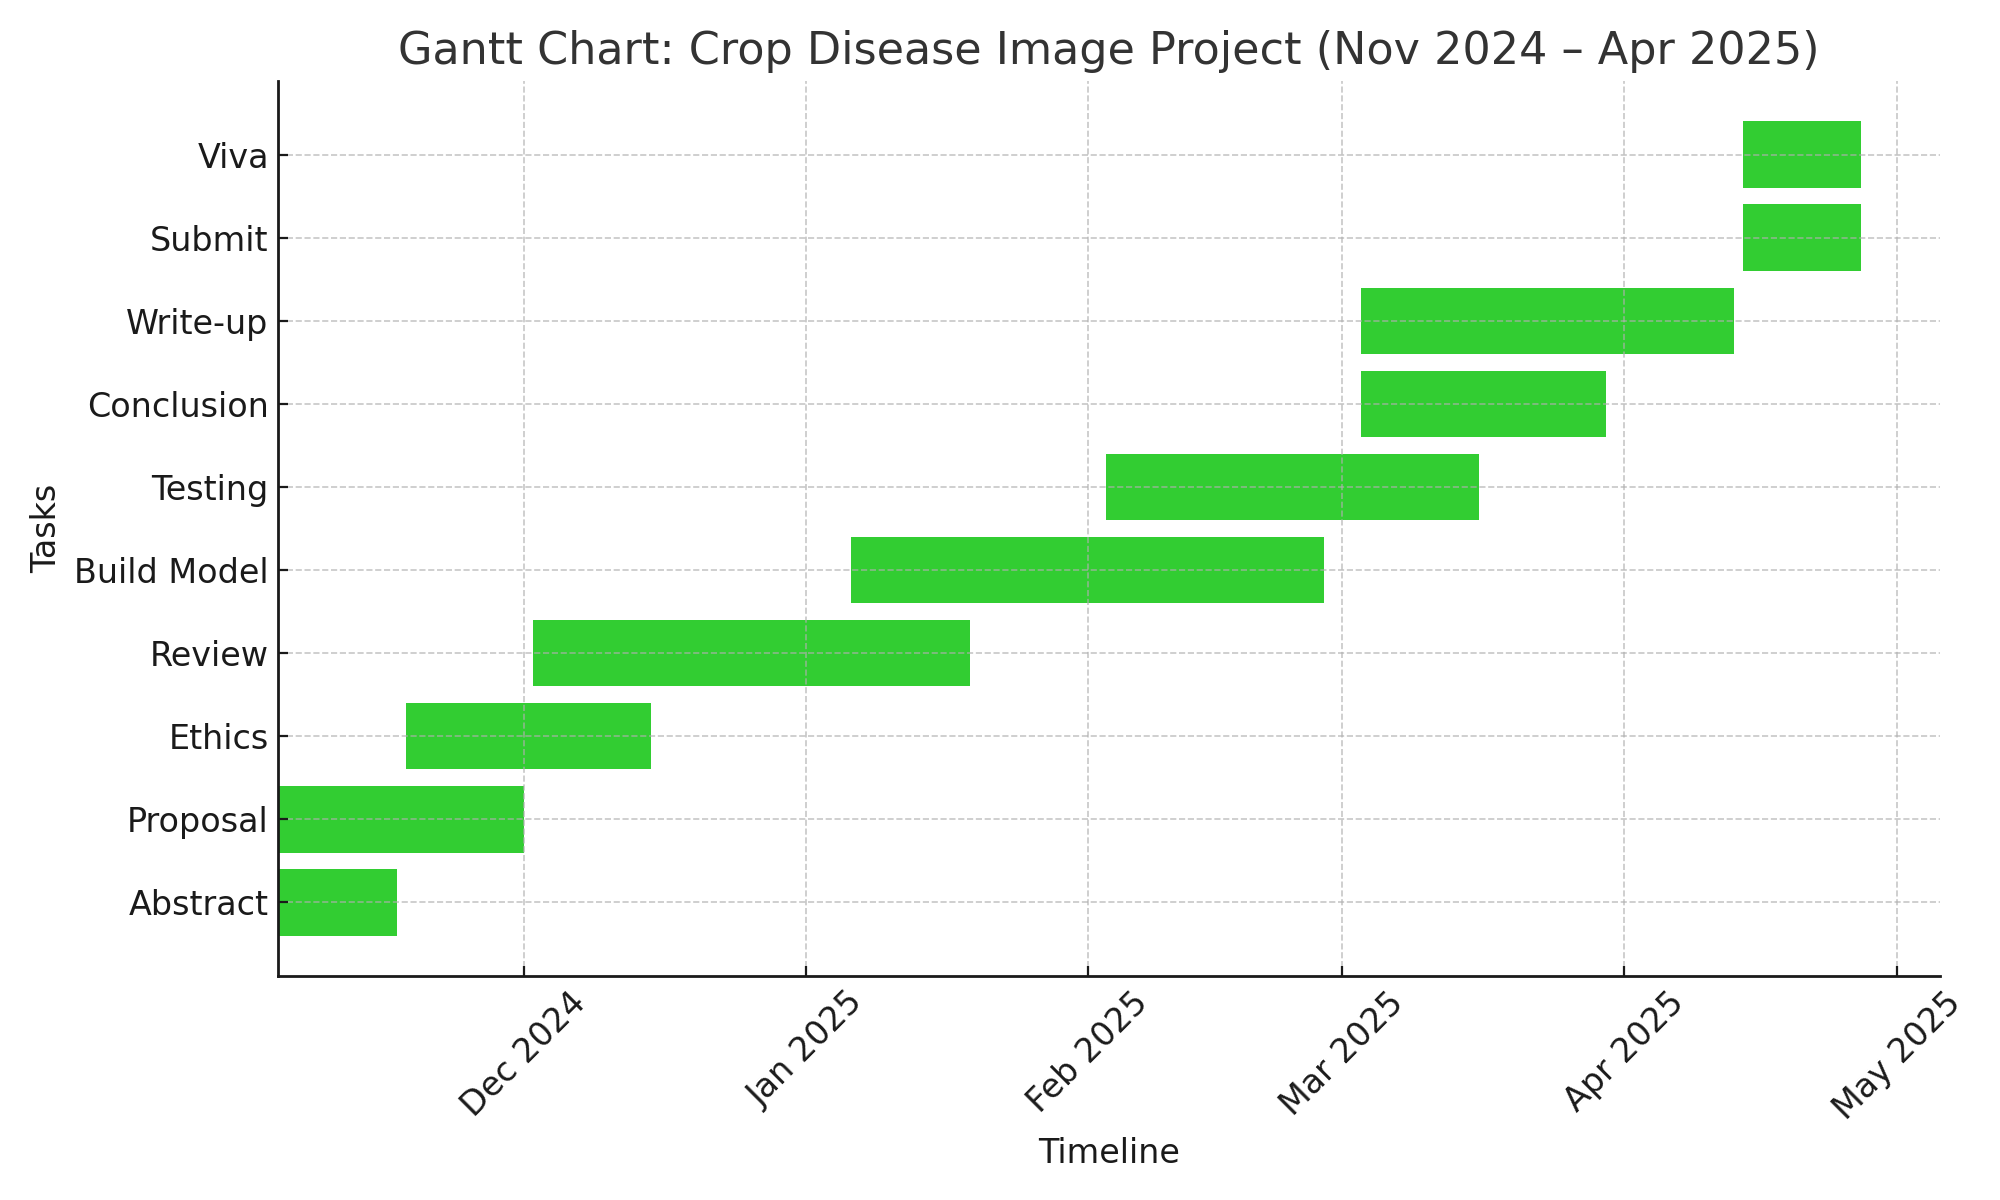
\includegraphics[width=0.95\textwidth]{figures/gantt_chart_project_limegreen.png}
    \caption{Gantt chart showing the timeline of the project}
    \label{fig:gantt_chart}
\end{figure}


% Bibliography
\clearpage
\renewcommand\bibname{References}
\addcontentsline{toc}{chapter}{Bibliography}
% Comment/uncomment as suits you
\bibliographystyle{IEEEtran} %% IEEE transaction style
% \bibliographystyle{acm} %% ACM style
% \bibliographystyle{alpha}
\bibliography{references}
\nocite{*}
\end{document}
